\documentclass[tikz,border=10pt]{standalone}
\begin{document}
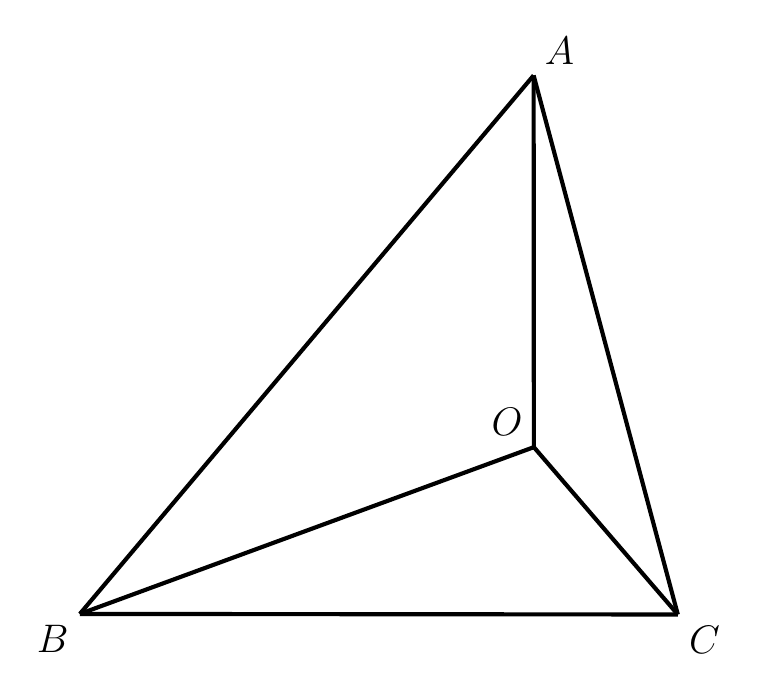
\begin{tikzpicture}[line join=round, line width=1.5pt]
\coordinate (A) at (1.964,3.435);
\coordinate (B) at (-3.799,-3.404);
\coordinate (C) at (3.795,-3.411);
\coordinate (O) at (1.967,-1.286);




\draw (A) -- (B);
\draw (B) -- (C);
\draw (A) -- (C);


\draw (A) -- (O);
\draw (B) -- (O);
\draw (O) -- (C);


\node[above right, font=\fontsize{15}{18}\selectfont] at (A) {$A$};
\node[below left, font=\fontsize{15}{18}\selectfont] at (B) {$B$};
\node[below right, font=\fontsize{15}{18}\selectfont] at (C) {$C$};
\node[above left, font=\fontsize{15}{18}\selectfont] at (O) {$O$};
\end{tikzpicture}
\end{document}